%%%%%%%%%%%%%%%%%%%%%%%%%%%%%%%%%%%%%%%%%
% baposter Landscape Poster
% LaTeX Template
% Version 1.0 (11/06/13)
%
% baposter Class Created by:
% Brian Amberg (baposter@brian-amberg.de)
%
% This template has been downloaded from:
% http://www.LaTeXTemplates.com
%
% License:
% CC BY-NC-SA 3.0 (http://creativecommons.org/licenses/by-nc-sa/3.0/)
%
%%%%%%%%%%%%%%%%%%%%%%%%%%%%%%%%%%%%%%%%%

%----------------------------------------------------------------------------------------
%	PACKAGES AND OTHER DOCUMENT CONFIGURATIONS
%----------------------------------------------------------------------------------------

\documentclass[landscape,a0paper,fontscale=0.285]{baposter} % Adjust the font scale/size here

\usepackage{graphicx} % Required for including images
\graphicspath{{figures/}} % Directory in which figures are stored

\usepackage{graphicx}
\usepackage{caption}
\usepackage{subcaption}
\usepackage{epstopdf}

\usepackage{amsmath} % For typesetting math
\usepackage{amssymb} % Adds new symbols to be used in math mode

\usepackage{booktabs} % Top and bottom rules for tables
\usepackage{enumitem} % Used to reduce itemize/enumerate spacing
\usepackage{palatino} % Use the Palatino font
\usepackage[font=small,labelfont=bf]{caption} % Required for specifying captions to tables and figures

\usepackage{multicol} % Required for multiple columns
\setlength{\columnsep}{1.5em} % Slightly increase the space between columns
\setlength{\columnseprule}{0mm} % No horizontal rule between columns

\usepackage{tikz} % Required for flow chart
\usetikzlibrary{shapes,arrows} % Tikz libraries required for the flow chart in the template

\newcommand{\compresslist}{ % Define a command to reduce spacing within itemize/enumerate environments, this is used right after \begin{itemize} or \begin{enumerate}
\setlength{\itemsep}{1pt}
\setlength{\parskip}{0pt}
\setlength{\parsep}{0pt}
}

\definecolor{lightblue}{rgb}{0.145,0.6666,1} % Defines the color used for content box headers

\begin{document}

\begin{poster}
{
columns=3,
headerborder=closed, % Adds a border around the header of content boxes
colspacing=1em, % Column spacing
bgColorOne=white, % Background color for the gradient on the left side of the poster
bgColorTwo=white, % Background color for the gradient on the right side of the poster
borderColor=lightblue, % Border color
headerColorOne=black, % Background color for the header in the content boxes (left side)
headerColorTwo=lightblue, % Background color for the header in the content boxes (right side)
headerFontColor=white, % Text color for the header text in the content boxes
boxColorOne=white, % Background color of the content boxes
textborder=roundedleft, % Format of the border around content boxes, can be: none, bars, coils, triangles, rectangle, rounded, roundedsmall, roundedright or faded
eyecatcher=true, % Set to false for ignoring the left logo in the title and move the title left
headerheight=0.1\textheight, % Height of the header
headershape=roundedright, % Specify the rounded corner in the content box headers, can be: rectangle, small-rounded, roundedright, roundedleft or rounded
headerfont=\Large\bf\textsc, % Large, bold and sans serif font in the headers of content boxes
%textfont={\setlength{\parindent}{1.5em}}, % Uncomment for paragraph indentation
linewidth=2pt % Width of the border lines around content boxes
}
%----------------------------------------------------------------------------------------
%	TITLE SECTION 
%----------------------------------------------------------------------------------------
%
{
\includegraphics[height=6em]{cde_tag_black.png}} % First university/lab logo on the left
{\bf\textsc{Doctor of Engineering (EngD) in Digital Entertainment, 1st year}\vspace{0.5em}} % Poster title
{\textsc{\{ Garoe Dorta Perez, Ieva Kazlauskaite and Richard Shaw \} \hspace{12pt} University of Bath}} % Author names and institution
{
\includegraphics[height=5em]{Bathlogo.jpg}} % Second university/lab logo on the right

%----------------------------------------------------------------------------------------
%	INVERSE KINEMATICS
%----------------------------------------------------------------------------------------

\headerbox{Inverse kinematics}{name=objectives,column=0,row=0}{

\begin{center}
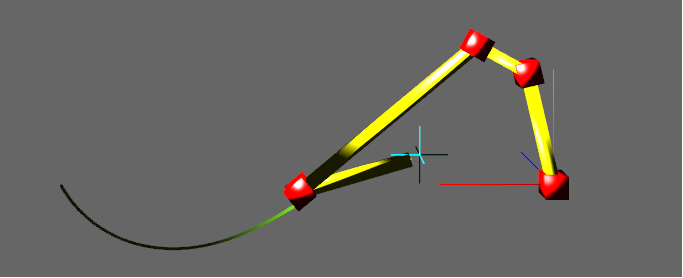
\includegraphics[width=0.8\linewidth]{chain3Dexamplev2}
\captionof{figure}{Linkage simulation with trace.}
\end{center}

Inverse kinematics uses a known end-effector position $\mathbf{E}$ to calculate the angles between the parts   $\boldsymbol\theta$ which ensure that the object reaches this desired target position, such that


where $f$ is the forward kinematics solver, $J$ is the Jacobian matrix and $J^+ = (J^T J)^{-1}J^T$ is the pseudoinverse of $J$.
\begin{equation*}
\begin{aligned}
\mathbf{E} &= f(\boldsymbol\theta) \rightarrow \boldsymbol{\theta} = f^{-1}(\mathbf{E}) \\  \partial \mathbf{E} &\approx J(\boldsymbol\theta) \partial \boldsymbol\theta \rightarrow \partial \boldsymbol{\theta} \approx J^{-1}(\partial\mathbf{E}),
\end{aligned}
\end{equation*}
where $f$ is the forward kinematics solver and $J$ is the Jacobian matrix.

\vspace{0.3em} % When there are two boxes, some whitespace may need to be added if the one on the right has more content
}

%----------------------------------------------------------------------------------------
%	FONT REGRESSION
%----------------------------------------------------------------------------------------

\headerbox{Font Regression}{name=introduction,column=1,row=0,bottomaligned=objectives}{
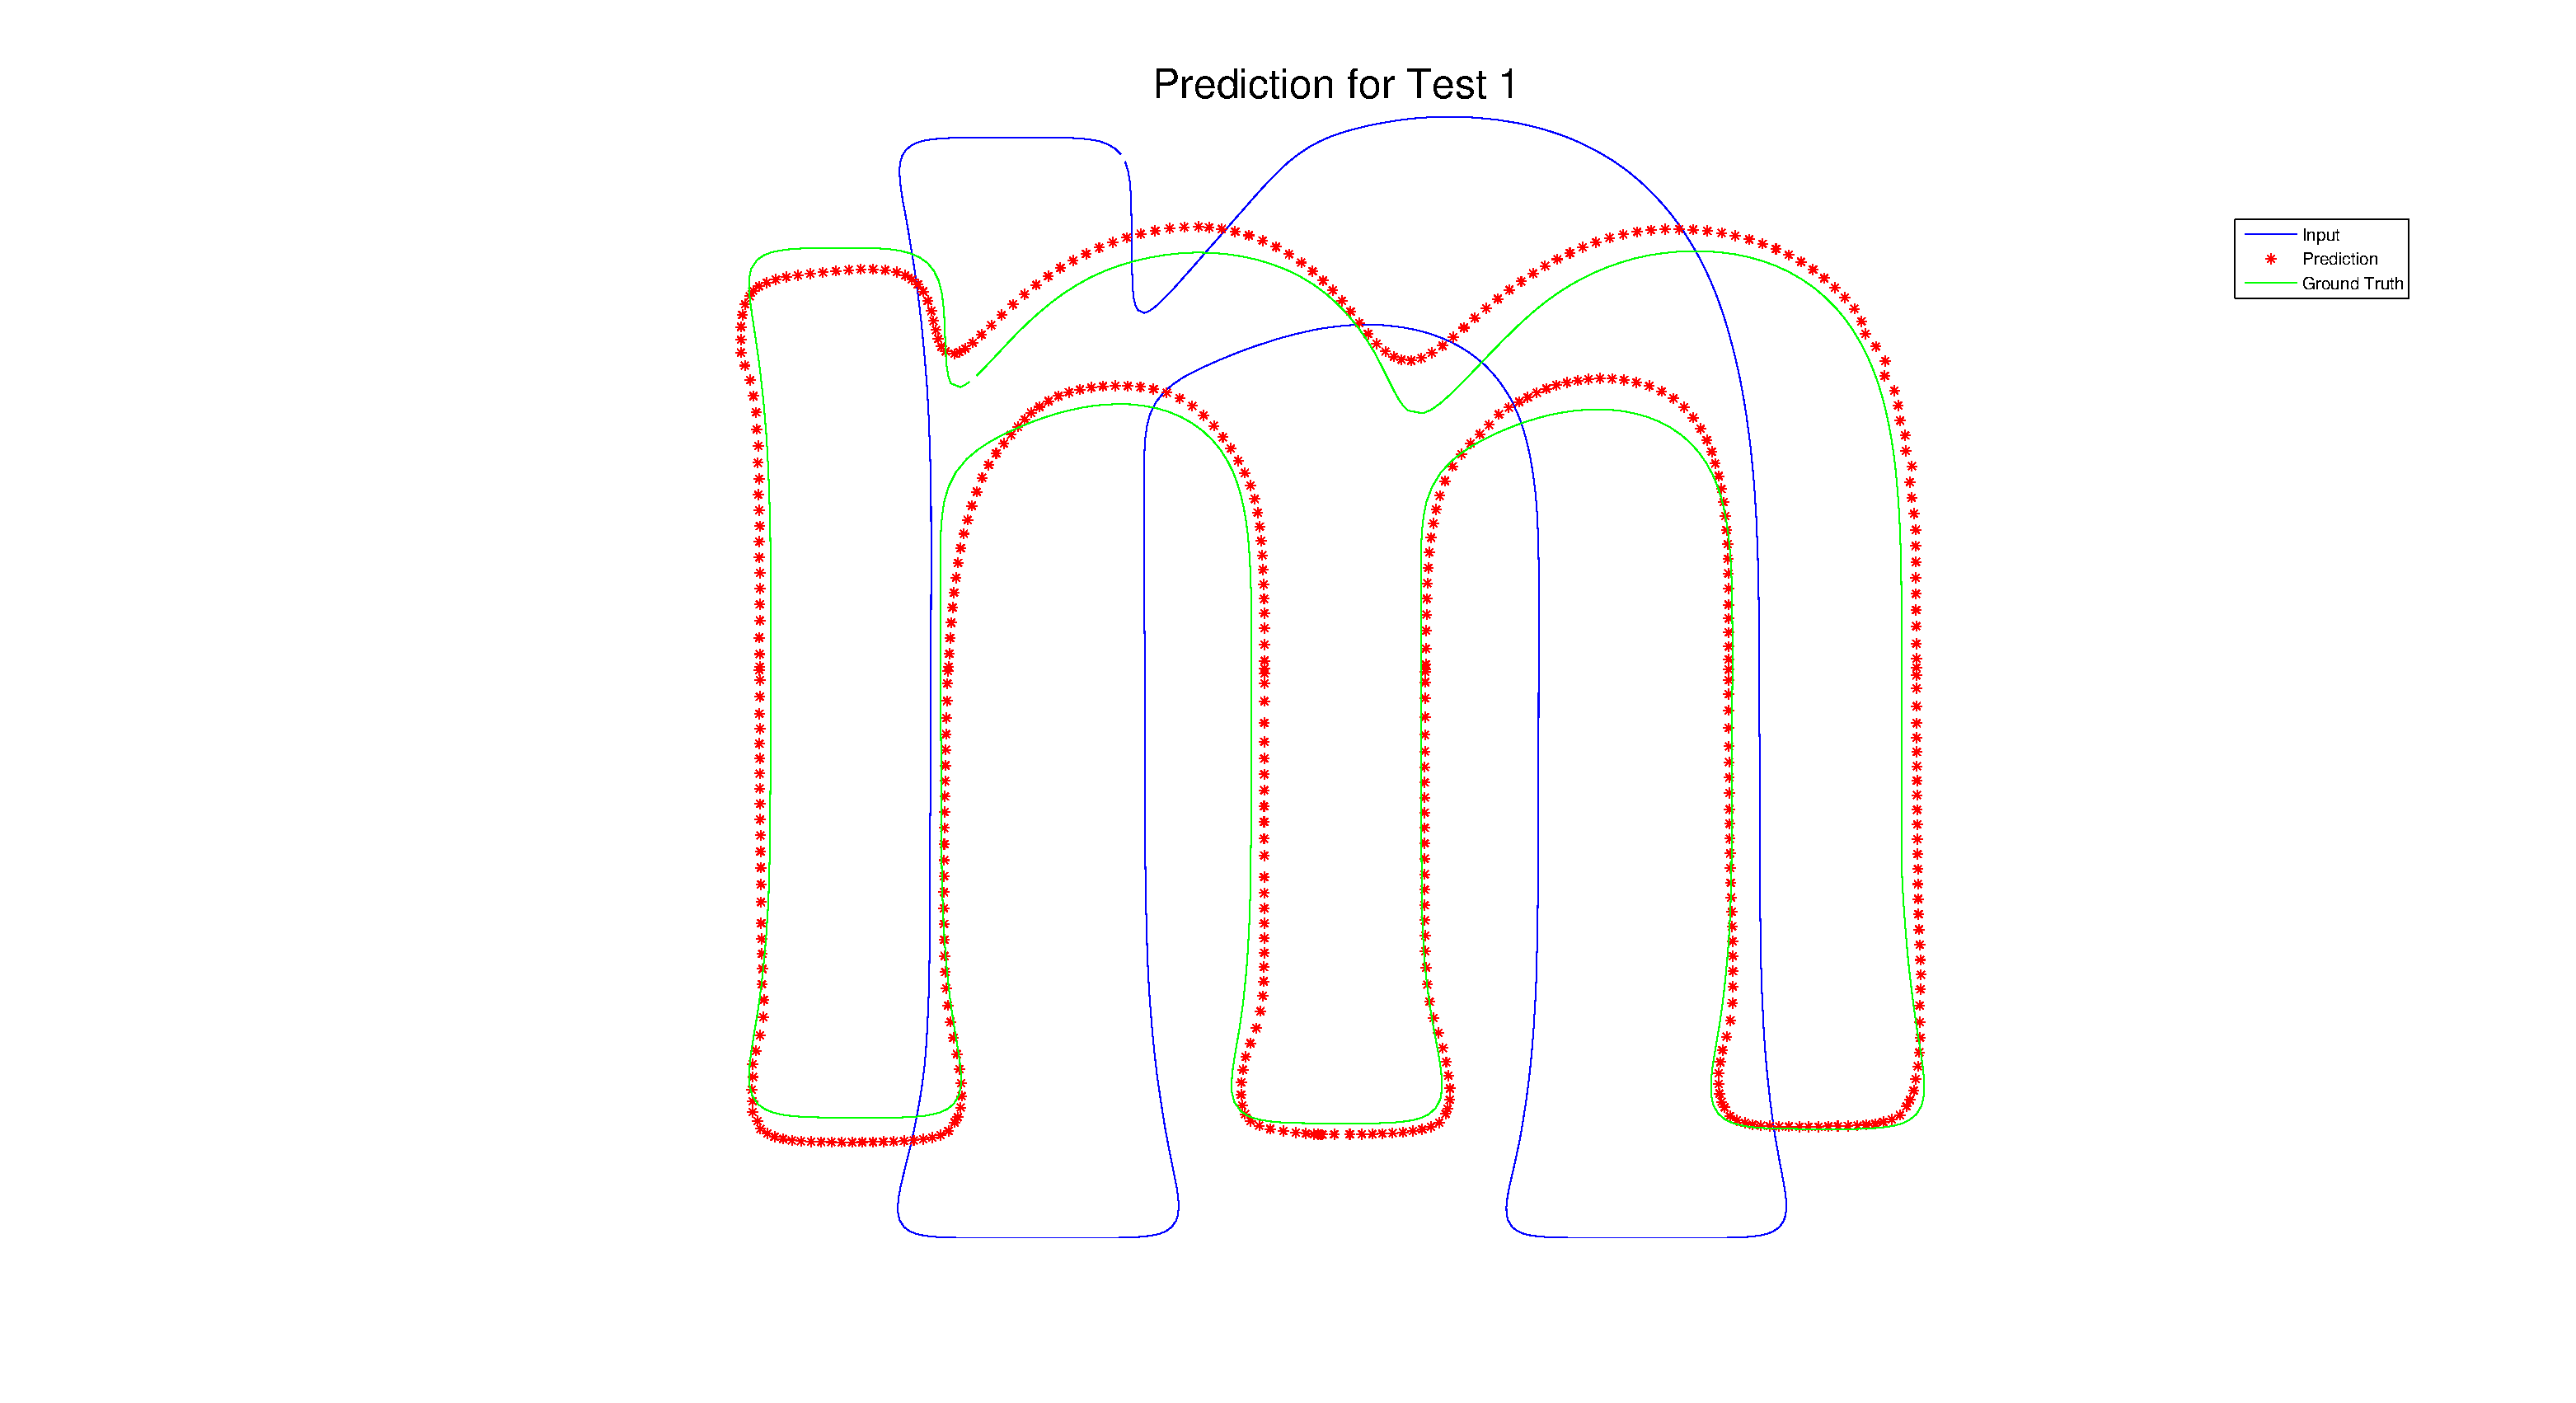
\includegraphics[trim = 120mm 20mm 120mm 20mm, clip, width=0.28\linewidth]{font1}
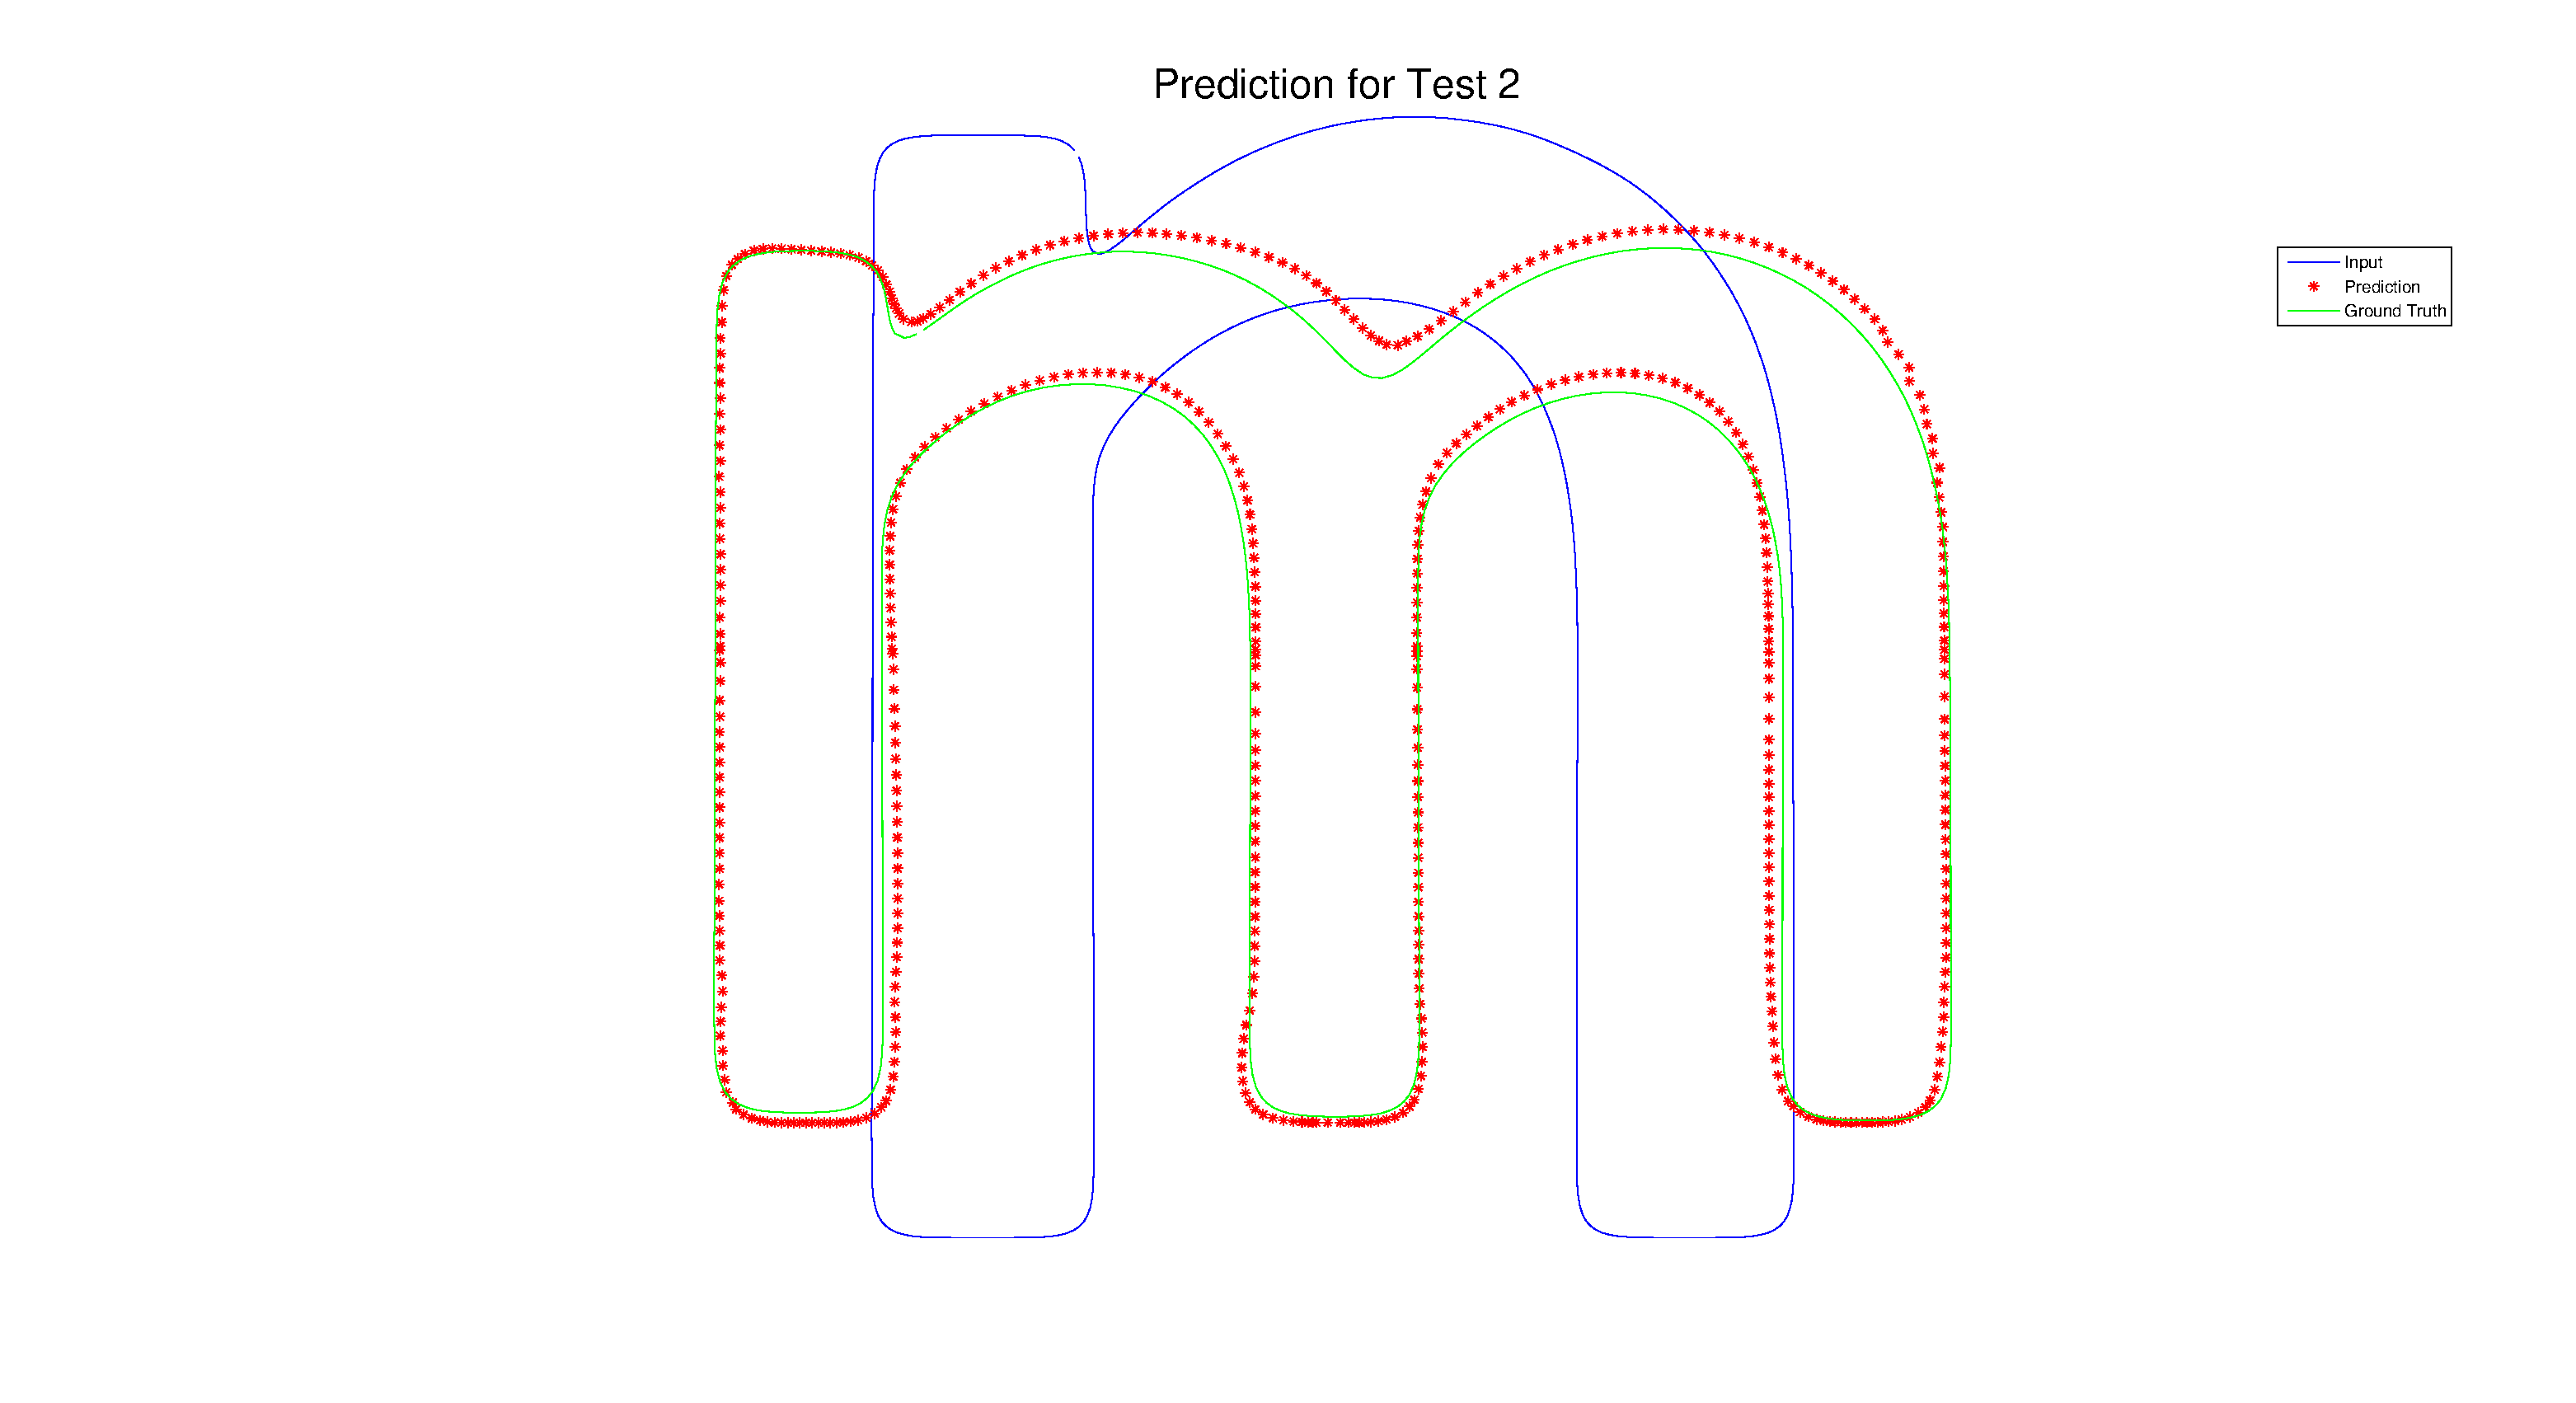
\includegraphics[trim = 120mm 20mm 120mm 20mm, clip,width=0.28\linewidth]{font2}
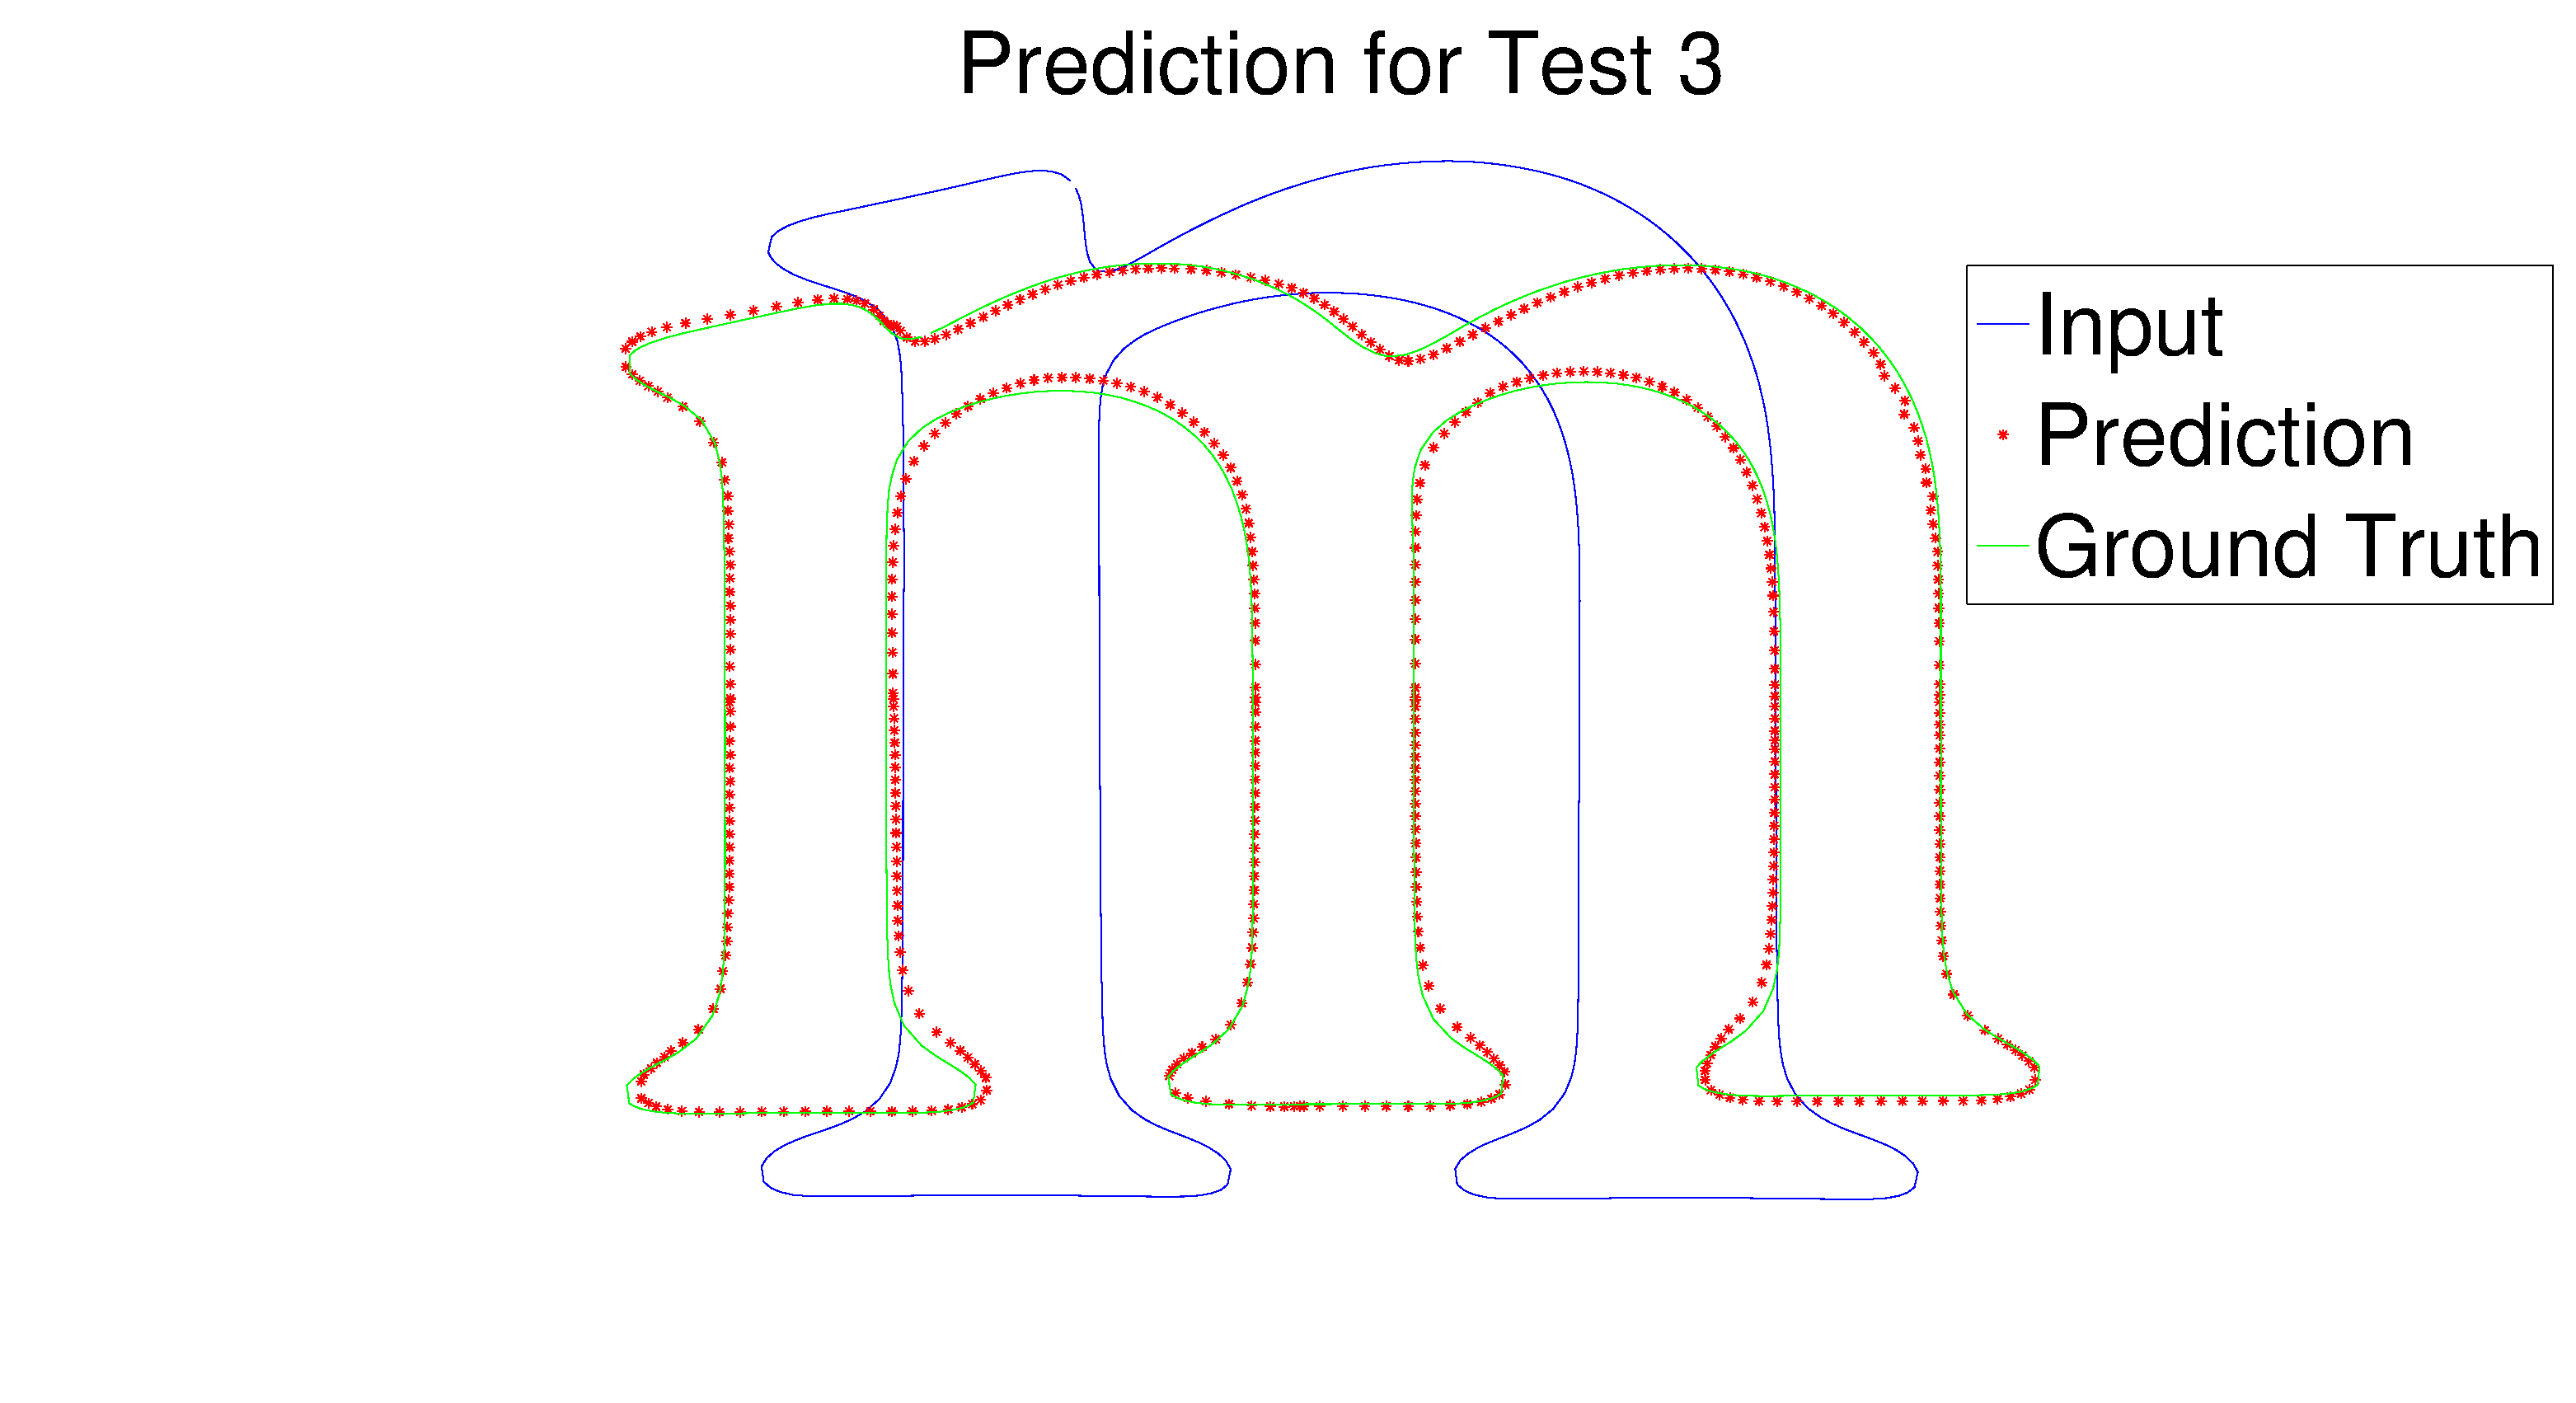
\includegraphics[trim = 120mm 20mm 0mm 20mm, clip,width=0.40\linewidth]{font3}
A Gaussian process is a random process, that can be considered as an infinite-dimensional generalisation of the multivariate Gaussian distribution. The main assumption of the Gaussian process modelling is that our data can be represented as a sample from a multivariate normal distribution. Each time a Gaussian process is used to model some data, a kernel has to be chosen, and its parameters tuned to maximise the likelihood. \\

Even with very few training examples, the Gaussian process model gives a reasonable prediction of the shape of a font. The best results were achieved using an exponential kernel with an optimised length scale and variance.
}

%----------------------------------------------------------------------------------------
%	SIFT
%----------------------------------------------------------------------------------------

\headerbox{SIFT Features}{name=results,column=2,span=1,row=0}{

Being able to detect features in an image that are invariant to scale, rotation, translation and changes in illumination has several applications.
SIFT features achieves the scale invariance through extrema detection in a difference of Gaussians pyramid built with the image, while the rotation dealt with an orientation assignment based on local image properties.

}

%----------------------------------------------------------------------------------------
%	REFERENCES
%----------------------------------------------------------------------------------------

\headerbox{References}{name=references,column=0,above=bottom}{

\renewcommand{\section}[2]{\vskip 0.05em} % Get rid of the default "References" section title
\nocite{*} % Insert publications even if they are not cited in the poster
\small{ % Reduce the font size in this block
\bibliographystyle{unsrt}
\bibliography{cde_poster} % Use sample.bib as the bibliography file
\vspace{1em}
}}

%----------------------------------------------------------------------------------------
%	FUTURE RESEARCH
%----------------------------------------------------------------------------------------

\headerbox{Future Research}{name=futureresearch,column=1,span=1,aligned=references,above=bottom}{ % This block is as tall as the references block

Integer sed lectus vel mauris euismod suscipit. Praesent a est a est ultricies pellentesque. Donec tincidunt, nunc in feugiat varius, lectus lectus auctor lorem, egestas molestie risus erat ut nibh.
\vspace{1em}
}

%----------------------------------------------------------------------------------------
%	CONTACT INFORMATION
%----------------------------------------------------------------------------------------

\headerbox{Contact Information}{name=contact,column=2,aligned=references,above=bottom}{ % This block is as tall as the references block

\begin{description}\compresslist
\item[Web] http://www.digital-entertainment.org
\item[Garoe Dorta Perez] g.dorta.perez@bath.ac.uk 
\item[Ieva Kazlauskaite] ik359@bath.ac.uk 
\item[Richard Shaw] richard.o.shaw@gmail.com
\end{description}
}


%----------------------------------------------------------------------------------------
%	PERFORMANCE-DRIVEN FACIAL ANIMATION
%----------------------------------------------------------------------------------------

\headerbox{Performance-driven Facial Animation}{name=conclusion,column=2,span=1,row=0,below=results,above=references}{

\begin{center}
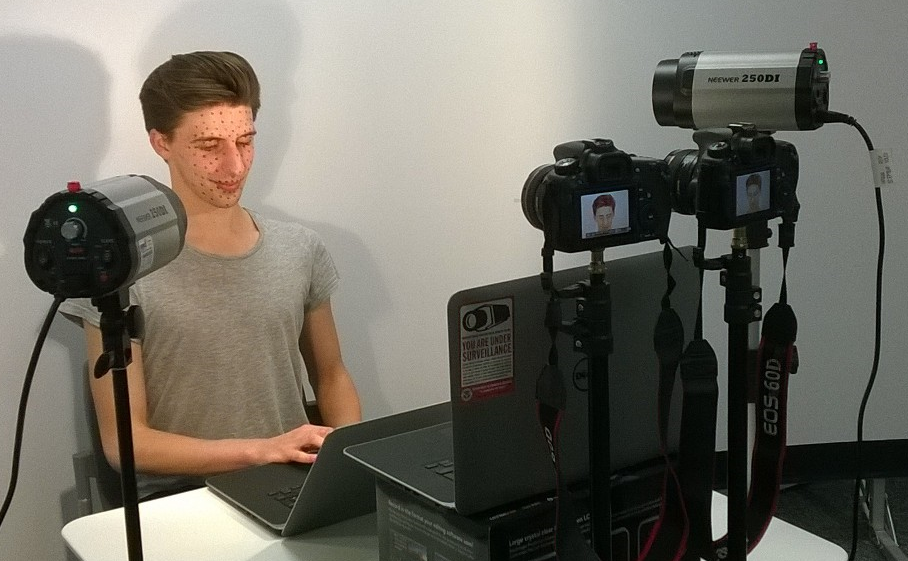
\includegraphics[width=0.5\linewidth]{facecapture}
\captionof{figure}{Linkage simulation with trace.}
\end{center}

\begin{center}
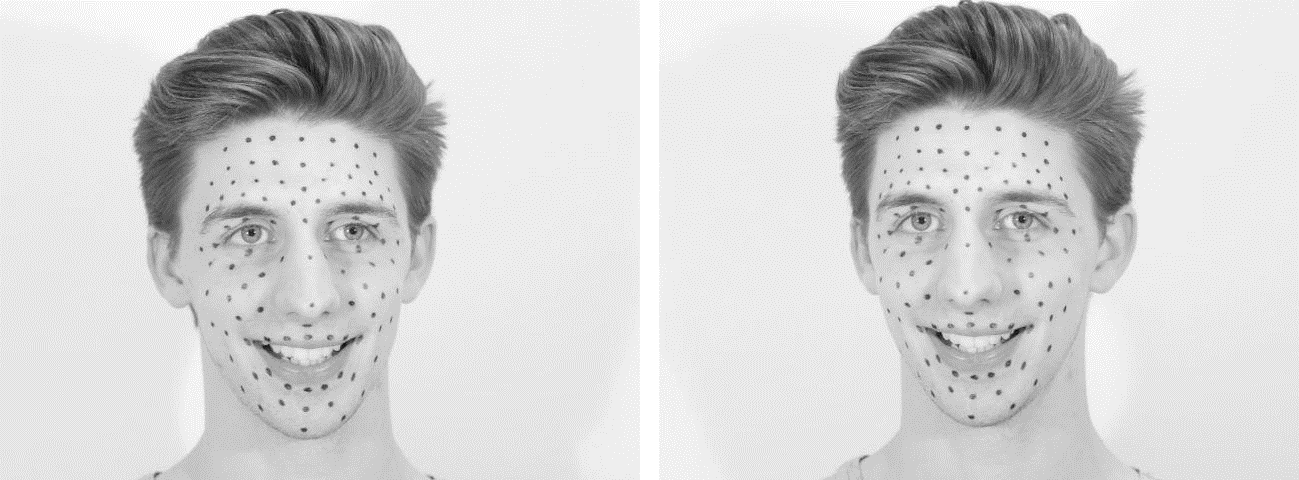
\includegraphics[width=0.8\linewidth]{stereoface}
\captionof{figure}{Linkage simulation with trace.}
\end{center}

A facial performance was captured using stereo cameras and by tracking markers on the face.


\begin{center}
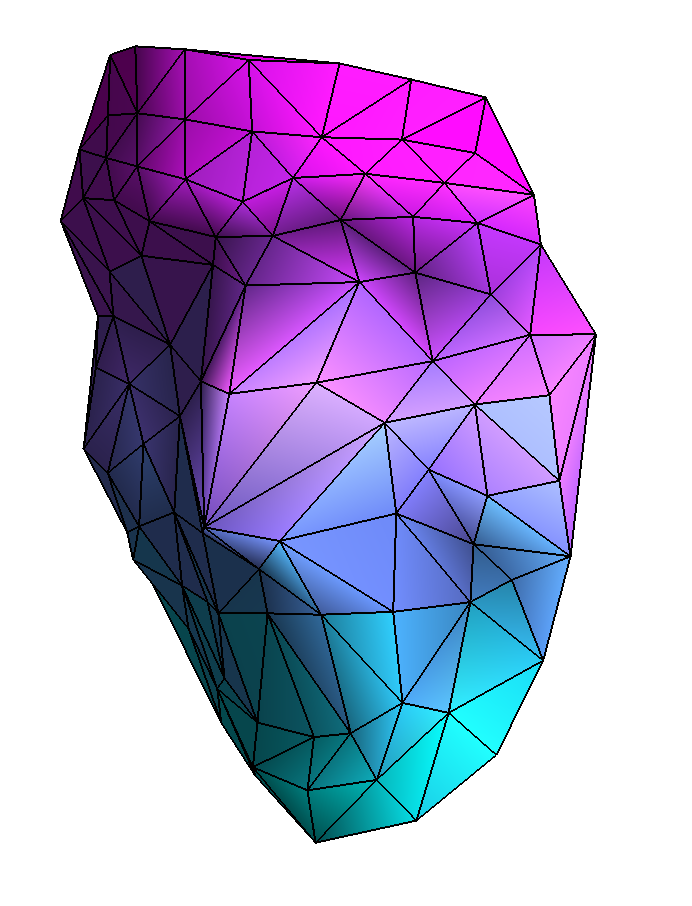
\includegraphics[width=0.4\linewidth]{face3d}
\captionof{figure}{Linkage simulation with trace.}
\end{center}

\begin{itemize}\compresslist
\item Pellentesque eget orci eros. Fusce ultricies, tellus et pellentesque fringilla, ante massa luctus libero, quis tristique purus urna nec nibh. Phasellus fermentum rutrum elementum. Nam quis justo lectus.
\end{itemize}

}

%----------------------------------------------------------------------------------------
%	SHAPE INTERPOLATION
%----------------------------------------------------------------------------------------

\headerbox{Shape interpolation}{name=method,column=0,below=objectives,bottomaligned=conclusion}{ % This block's bottom aligns with the bottom of the conclusion block
Alexa et al~\cite{Alexa:2000} introduced a transformation-based interpolation technique, that aims to preserve the structure of the parts that are only translated or rotated between the two meshes. For each triangle the transformation \(mathbf{A}\) is split into rotation and translation/shearing; then the angles and the scale/shearing are transformed linearly. The mapping that is close to \(\mathbf{a}\) and that transforms the vertices smoothly is found by minimising the error:
\begin{equation}
	E_{V(t)} = \sum_{T \in \mathcal{T}} || A_T(t) - B_T(t)||^2_F,\label{eq:error}
\end{equation} 
where \(\mathcal{T}\) is the triangulation, and \(|| \cdot ||^2_F \) is the Frobenius norm. The new transformation matrix \(B\) is defined in terms of the intermediate position of the vertices \(V(t) = (\mathbf{v}_1(t), \dots, \mathbf{v}_n(t))\) such that \(V(0)\) is the initial position of the vertices and \(V(1)\) is the final position. Consequently,
\begin{equation}
	B_T (t) \: \mathbf{p}_f + \mathbf{l} = \mathbf{v}_f(t), \: f \in \{i,j,k\}.\label{eq:B}
\end{equation} 


}

%----------------------------------------------------------------------------------------
%	3D RECONSTRUCTION
%----------------------------------------------------------------------------------------

\headerbox{3D Reconstruction}{name=results2,column=1,below=objectives,bottomaligned=conclusion}{ % This block's bottom aligns with the bottom of the conclusion block



}

%----------------------------------------------------------------------------------------

\end{poster}

\end{document}